\section{Dataset Summary} \label{datasummary}
Our dataset contains sketches, their semantic part annotations, and descriptions for every part in a sketch. 
The sketches comes from the QuickDraw dataset \citep{ha2017neural}, and the semantic part annotations come from the SPG dataset \citep{spg_paper}; both datasets are explained in details in Section \ref{relatedWorkChapter}.

We annotated for 2 categories of sketches: face and angel. 
For angel sketches, we annotate for the parts \textit{halo}, \textit{eyes}, \textit{nose}, \textit{mouth}, \textit{body}, \textit{outline of face}, and \textit{wings}. 
For face sketches, we annotate for the parts \textit{eyes}, \textit{nose}, \textit{mouth}, \textit{hair}, \textit{outline of face}. 


\begin{table}[!htb]
\begin{minipage}{1\textwidth}
\begin{center}
{\small
\begin{tabular}{lrrr}
\toprule
~ & Face & Angel \\
\midrule
Number of contrasting pairs & 2515 & 3060 \\
Number of distinct words & 833 & 1107 \\
Number of sketches & 572 & 787 \\
\bottomrule
\end{tabular}}
\caption{Dataset statistics by category.}
\label{table:dataset_stats1}
\end{center}
\end{minipage}
\end{table}

\begin{table}[!htb]
\begin{minipage}{1\textwidth}
\begin{center}
{\small
\begin{tabular}{p{9em} | p{1.5em}p{1.5em}p{2em}p{1.5em}p{1.5em} | p{1.5em}p{1.5em}p{1.5em}p{2em}p{1.5em}p{1.5em}p{1.5em} }
\toprule
~ & \multicolumn{5}{c}{Face} & \multicolumn{7}{c}{Angel}\\
~ & eyes & nose & mouth & hair & face & halo & eyes & nose & mouth & face & body & wings  \\
\midrule
Number of sketches & 
334 & 572 & 572 & 104 & 572 &
558 & 114 & 8 & 80 & 732 & 781 & 779 \\
Number of distinct words & 
228 & 360 & 325 & 152 & 314 & 
365 & 112 & 21 & 88 & 379 & 425 & 534 \\
Number of contrasting pairs &
689 & 401 & 687 & 126 & 612 &
559 & 114 & 8 & 80 & 733 & 785 & 781 \\
\bottomrule
\end{tabular}}
\caption{Dataset statistics by sketch parts. The phrase \textit{contrasting pair} refers to a pair of sketches with contrasting features that are presented to the annotators.}
\label{table:dataset_stats_byparts}
\end{center}
\end{minipage}
\end{table}

\begin{figure*}[!htb]
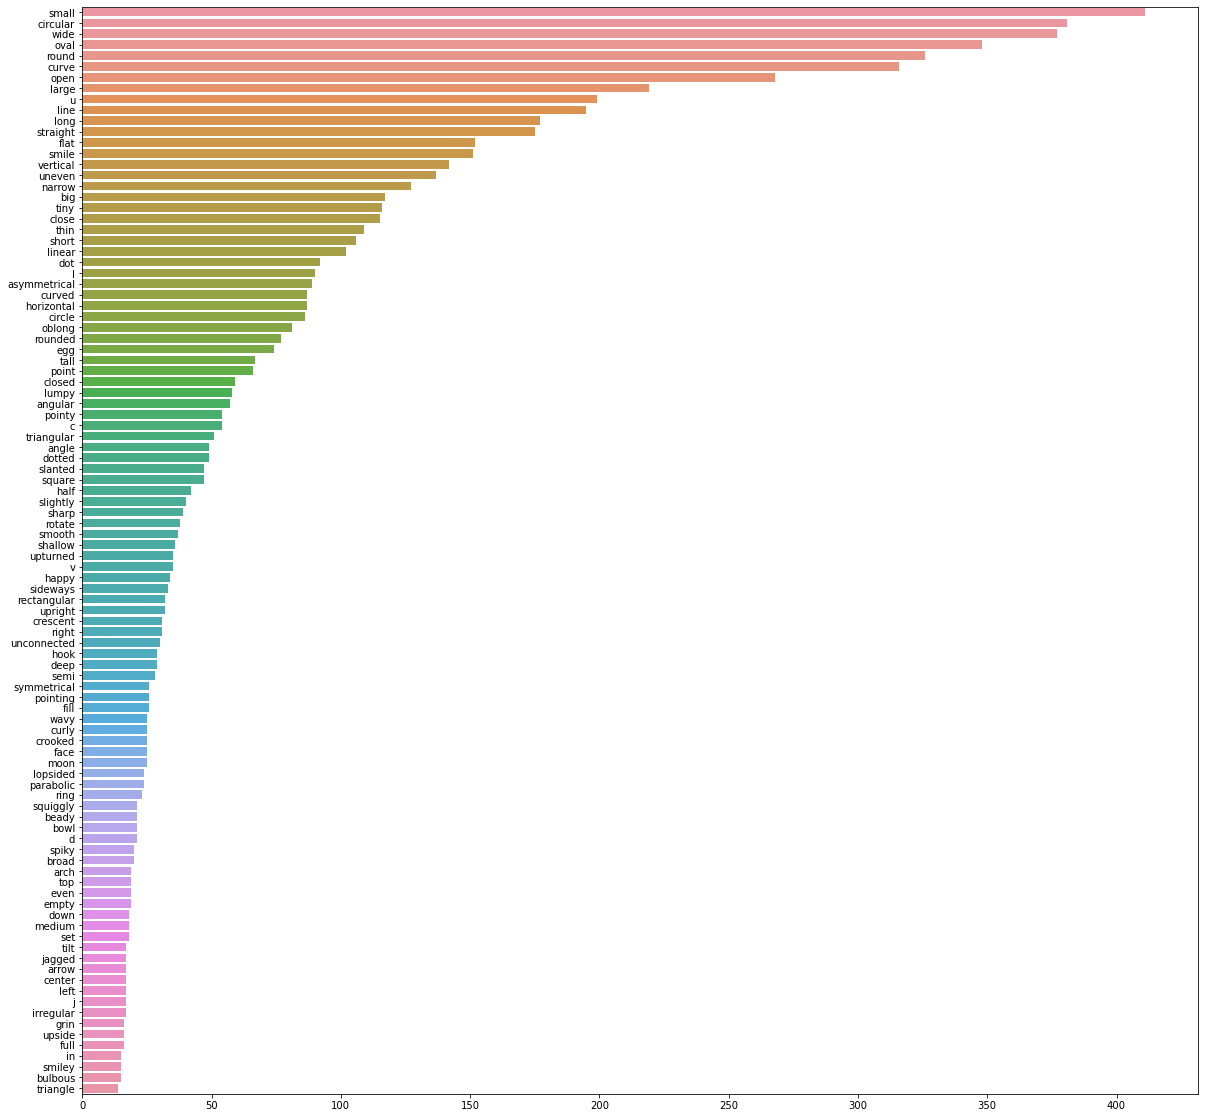
\includegraphics[width=\linewidth]{dataset_image/word_freq_face.png}  
\caption{Top 100 most frequent words in the dataset corpus. X-axis: number of descriptions containing the word.}
\label{word_freq}
\end{figure*}

In Table \ref{table:dataset_stats_byparts}, we present dataset statistics broken down by semantic parts, and, in Table \ref{table:dataset_stats1}, we show the same statistics by sketch category. In Figure \ref{word_freq}, we show 100 most frequently used words in our dataset. 

% \subsection{Compare with DoodlerGAN Dataset}
The \textit{Creative Birds} and \textit{Creative Creatures} datasets collected by DoodlerGAN \citep{doodlerGAN} contain 2 categories, like ours, but there are 9k sketches in each category, and ours contains one tenth as many. Although we fall short on the number of sketches and the variety of sketching styles, we approach creativity from a completely different angle: we focus on how people compose similar basic shapes to create sketches of different categories and adapt similar language to describe different sketch parts, as explained in Section \ref{introductionChapter} and Figure \ref{introduction.composition}.  

\begin{figure*}[!htb]
\begin{subfigure}{\textwidth}
\centering
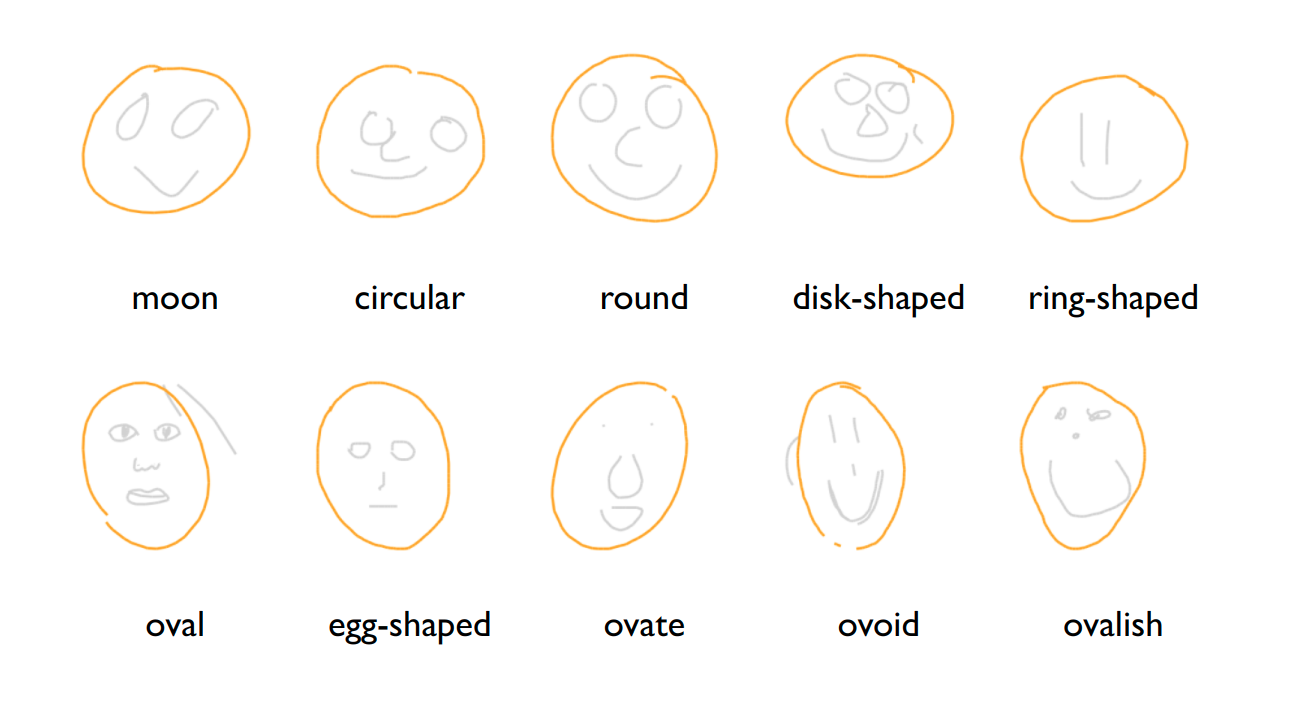
\includegraphics[width=\linewidth]{data_collection/summary/circles_descriptions.png}  
\end{subfigure}
\caption{Different ways of describing circles (top) and ovals (bottom) in the dataset.}
\label{datasummary.circles.varied_language}
\end{figure*}

Our face sketches contain 5 different parts, and angel sketches have 7 parts; there are 7 parts in Creative Birds and 16 parts in Creative Creatures. Again, we do not annotate for as many parts as DoodlerGAN. 
However, in our dataset, every part in every sketch has at least 2 different language annotations describing the visual features, while DoodlerGAN has no language annotation. 
With text descriptions, in addition to part-based generative model, we can study how to generate similar shapes from different text descriptions. In Figure \ref{datasummary.circles.varied_language}, we show how people describe \textit{circles} using various descriptors (the figure only contains a subset of ways describing circles).  
In Figure \ref{datasummary.face.varied_language}, we show the variety of language in describing a simple smiley face. Similarly, an example of creative description of different parts in angel sketches is shown in Figure \ref{datasummary.angel.varied_language}.  


\begin{figure*}[!htb]
\begin{subfigure}{\textwidth}
\centering
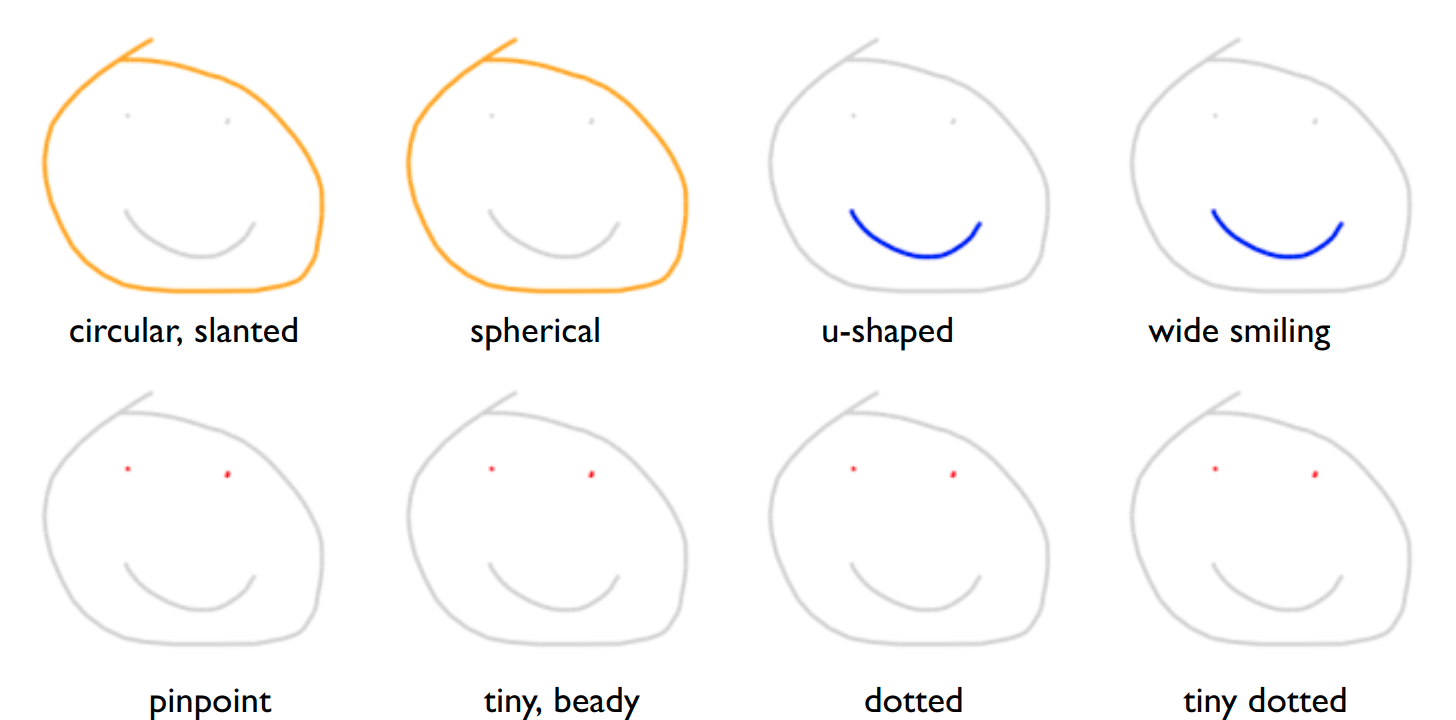
\includegraphics[width=\linewidth]{data_collection/summary/smileyface_descriptions.png}  
\caption{Each part in this simple face sketch receives at least 2 descriptions from different annotators.}
\label{datasummary.face.varied_language}
\end{subfigure}
\newline
\begin{subfigure}{\textwidth}
\centering
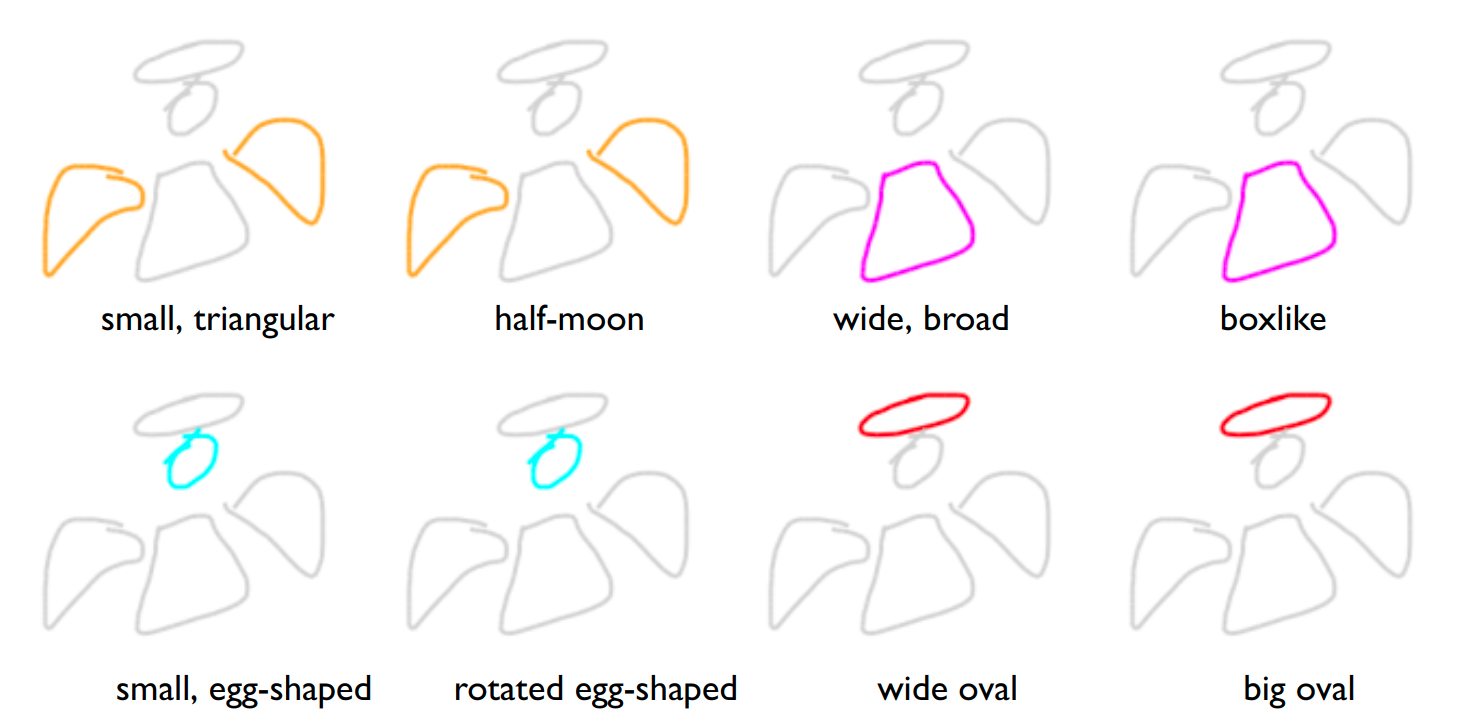
\includegraphics[width=\linewidth]{data_collection/summary/angel_descriptions.png}  
\caption{An example of diverse descriptions for each part in the angel sketch.}
\label{datasummary.angel.varied_language}
\end{subfigure}
\caption{Two examples from the face and angel categories that illustrate our dataset containing creative descriptions of sketches despite their simplicity. The caption at the bottom of each image is provided by annotators to describe the highlighted part in the sketch. For example, the wings are described as either \textit{small, triangular} or \textit{half-moon}.}
\label{datasummary.face_angel.varied_language}
\end{figure*}
% In general, we observe that compared to previous work that tend to have a fixed list of adjectives for each object parts, the descriptions in our dataset are free-form and non-constrainted. This characteristics is desirable and aligns with our goal to allow robot to collaborate smoothly with humans, since different people would describe the same things in very diverse ways. 

% \subsection{Compare with SketchCUB Dataset}
% SketchCUB contains both sketch and language annotations \citep{sketchbirds}. However, it predetermines 312 binary attributes 


\begin{table}[!htb]
\begin{minipage}{1\textwidth}
\begin{center}
{\small
\begin{tabular}{p{5em} | p{1.5em}p{1.5em}p{2em}p{1.5em}p{1.5em} | p{1.5em}p{1.5em}p{1.5em}p{2em}p{1.5em}p{1.5em}p{1.5em} }
\toprule
~ & \multicolumn{5}{c}{Face} & \multicolumn{7}{c}{Angel}\\
~ & eyes & nose & mouth & hair & face & halo & eyes & nose & mouth & face & body & wings  \\
\midrule
small & 192 & 143 & 65 & 2 & 9 & 150 & 53 & 8 & 25 & 202 & 64 & 47 \\
oval & 123 & 7 & 11 &   & 207 & 258 & 1 &   &   & 145 & 42 & 23 \\
circular & 164 & 12 & 11 & 2 & 192 & 80 & 14 & 1 & 2 & 276 & 10 & 11 \\
round & 175 & 18 & 2 & 1 & 130 & 91 & 8 &   &   & 268 & 22 & 45 \\
wide & 94 & 16 & 193 &   & 74 & 84 & 2 &   & 12 & 50 & 120 & 111 \\
open & 118 & 7 & 106 &   & 37 & 54 & 6 &   & 1 & 79 & 137 & 26 \\
large & 98 & 41 & 58 &   & 22 & 66 & 6 &   &   & 131 & 54 & 85 \\
curve & 23 & 52 & 221 & 3 & 17 & 18 & 9 & 1 & 27 & 10 & 58 & 101 \\
triangular & 9 & 20 & 9 & 2 & 11 & 10 &   &   &   & 14 & 294 & 42 \\
line & 92 & 27 & 56 & 19 & 1 & 15 & 22 & 3 & 14 & 3 & 93 & 9\\
\bottomrule
\end{tabular}}
\caption{This table shows how many times each of the top-10 most frequently used word in the dataset is used to describe different parts in face and angel sketches. For example, \textit{small} is used in 192 descriptions for eyes in face sketches, and it is used 150 times to describe angel halos. People use the same words differently depending on the sketching context.}
\label{table:parts_share_description}
\end{center}
\end{minipage}
\end{table}

Moreover, using this dataset, we can study how people compose concepts (e.g. \textit{large}$+$\textit{round}) and apply the same concepts to different semantic parts (e.g. \textit{large round eyes} and \textit{large round halo}).     
We observe that face and angel sketches share 486 words in total, and for the 200 words that occur most frequently in the dataset (all used in at least 13 part descriptions), 182 are shared across the two categories. Therefore, we believe that the datasets would allow us to study how people use similar words when sketching different objects. Although we cannot conclude in this project, we have already found some examples of the meaning of descriptors varied across sketches, after examining a few words. Figure \ref{datasummary.spiky} shows an example. In this example, \textit{spiky} is used to mean either short hair in face sketches or pointy, edgy wings in angel sketches. Moreover, there is an implicit orientation change between the two categories of sketches: while \textit{spiky hair} implies ``spike'' in the vertical direction, the phrase, \textit{spiky wings}, implies jigsaws pointing out from the angel body, horizontally.   

\begin{figure*}[!htb]
\begin{subfigure}{.5\textwidth}
\centering
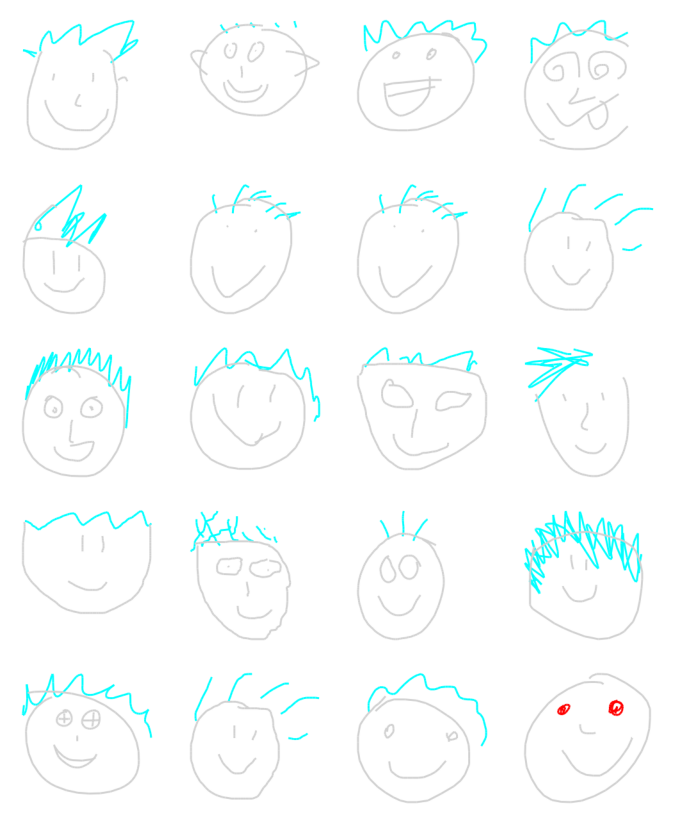
\includegraphics[width=0.9\linewidth]{data_collection/summary/spikyface.png}  
% \caption{Face sketches whose hair description contains the word \textit{spiky}. In this case, the word refers to short and coarse texture of hair.}
% \label{datasummary.spiky.face}
\end{subfigure}
\hspace{5mm}
\begin{subfigure}{.5\textwidth}
\centering
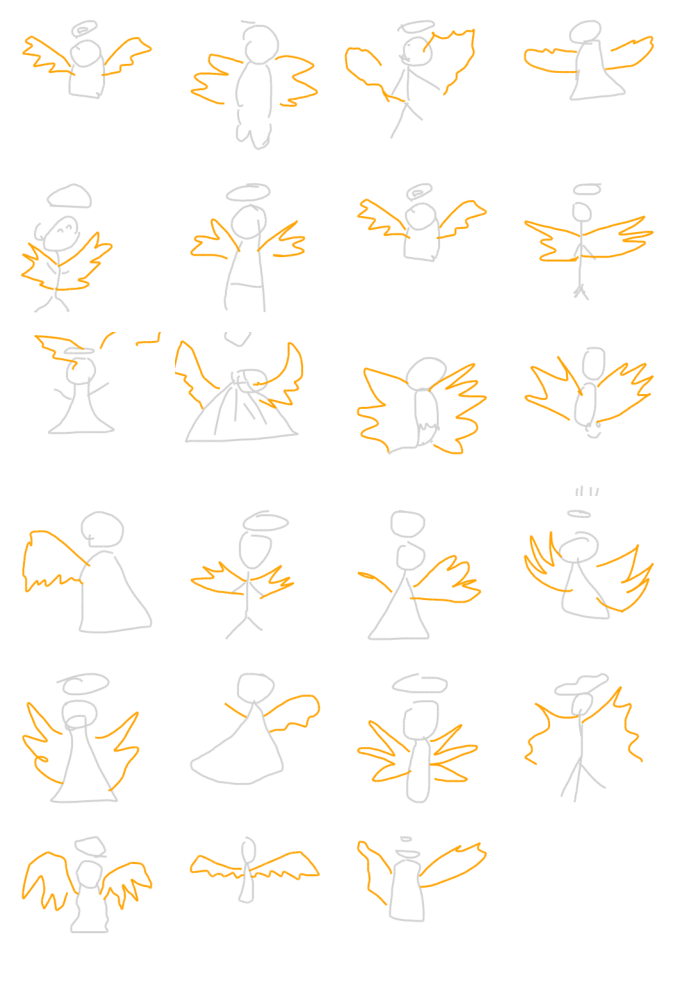
\includegraphics[width=\linewidth]{data_collection/summary/spikyangel.png}  
% \caption{Angel sketches whose wing description contains the word \textit{spiky}, which is used to represent the pointy edges on wings.}
% \label{datasummary.spiky.angel}
\end{subfigure}
\caption{Left: face sketches whose hair descriptions contain the word \textit{spiky}. In faces, the word refers to short and coarse texture of hair. Right: angel sketches whose wing description contains the word \textit{spiky}, which is used to represent the pointy edges on wings.}
\label{datasummary.spiky}
\end{figure*}